\documentclass[10pt]{article}
\usepackage{pgf,tikz}
\usetikzlibrary{arrows}
\pagestyle{empty}
\begin{document}
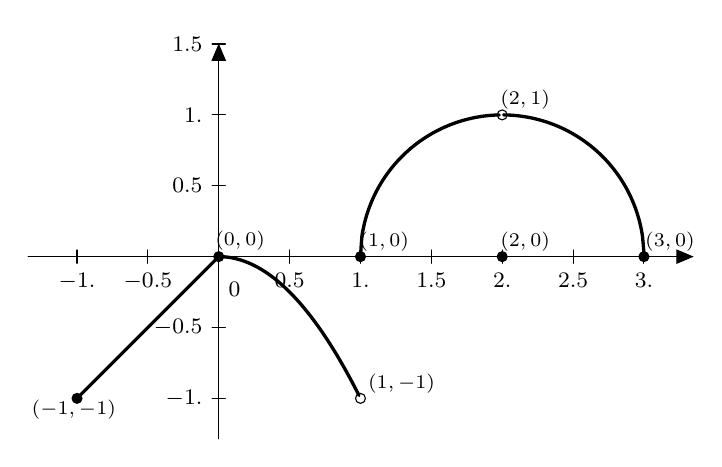
\begin{tikzpicture}[scale=1.2,line cap=round,line join=round,>=triangle 45,x=1.5cm,y=1.5cm]
\draw[->,color=black] (-1.34420610852,0.) -- (3.35070584374,0.);
\foreach \x in {-1.,-0.5,0.5,1.,1.5,2.,2.5,3.}
\draw[shift={(\x,0)},color=black] (0pt,2pt) -- (0pt,-2pt) node[below] {\footnotesize $\x$};
\draw[->,color=black] (0.,-1.28480272013) -- (0.,1.50373574833);
\foreach \y in {-1.,-0.5,0.5,1.,1.5}
\draw[shift={(0,\y)},color=black] (2pt,0pt) -- (-2pt,0pt) node[left] {\footnotesize $\y$};
\draw[color=black] (0pt,-10pt) node[right] {\footnotesize $0$};
\clip(-1.34420610852,-1.28480272013) rectangle (3.35070584374,1.50373574833);
\draw[line width=1.2pt,smooth,samples=100,domain=-1.0:0.0] plot(\x,{(\x)});
\draw[line width=1.2pt,smooth,samples=100,domain=0.0:0.99] plot(\x,{0-(\x)^(2.0)});
\draw[line width=1.2pt,smooth,samples=100,domain=1.0:1.98] plot(\x,{sqrt(1.0-((\x)-2.0)^(2.0))});
\draw[line width=1.2pt,smooth,samples=100,domain=2.01:3.0] plot(\x,{sqrt(1.0-((\x)-2.0)^(2.0))});
\begin{scriptsize}
\draw [fill=black] (0.,0.) circle (1.5pt);
\draw[color=black] (0.150988780732,0.113204501323) node {$(0, 0)$};
\draw [fill=black] (-1.,-1.) circle (1.5pt);
\draw[color=black] (-1.02273920733,-1.08295141008) node {$(-1, -1)$};
\draw [color=black] (1.,-1.) circle (1.5pt);
\draw[color=black] (1.29014922876,-0.896052048923) node {$(1, -1)$};
\draw [fill=black] (1.,0.) circle (1.5pt);
\draw[color=black] (1.16772130542,0.105728526877) node {$(1, 0)$};
\draw [fill=black] (2.,0.) circle (1.5pt);
\draw[color=black] (2.16202590678,0.105728526877) node {$(2, 0)$};
\draw [color=black] (2.,1.) circle (1.5pt);
\draw[color=black] (2.16202590678,1.10750910268) node {$(2, 1)$};
\draw [fill=black] (3.,0.) circle (1.5pt);
\draw[color=black] (3.18380648258,0.105728526877) node {$(3, 0)$};
\end{scriptsize}
\end{tikzpicture}
\end{document}